\documentclass[a4paper, 12pt]{article}%тип документа

%отступы
\usepackage[left=2cm,right=2cm,top=2cm,bottom=3cm,bindingoffset=0cm]{geometry}

%Русский язык
\usepackage[T2A]{fontenc} %кодировка
\usepackage[utf8]{inputenc} %кодировка исходного кода
\usepackage[english,russian]{babel} %локализация и переносы

%Вставка картинок
\usepackage{wrapfig}
\usepackage{graphicx}
\graphicspath{{pictures/}}
\DeclareGraphicsExtensions{.pdf,.png,.jpg}

%Графики
\usepackage{multirow}
\usepackage{pgfplots}
\usepackage{rotating}
\usepackage{pgfplotstable}
\usepackage{booktabs}
\usepackage{multirow}
\pgfplotsset{compat=1.9}

%Математика
\usepackage{amsmath, amsfonts, amssymb, amsthm, mathtools}

%Заголовок
\author{Сифат Мд Абдуллах Ал Хасиб \\
Физтех школа электроники, фотоники и молекулярной физики \\
Группа Б04-105}
\title{\textbf{Лаборатория Работа 2.2.1 \\ 
Исследование взаимной диффузии газов}}
\begin{document}
\maketitle
\section{Введение}\textbf{Цель работы:}Регистрация  зависимости  концентрации   гелия в воздухе от времени с помощью датчиков теплопроводности при разных начальных давлениях смеси газов; 2) определение коэффициента диффузии по результатам измерений.\\
\textbf{В работе используется:}Измерительная установка; форвакуумный насос; баллон с газом (гелий); манометр; источник питания; магазин сопротивлений; гальванометр; секундомер.
\section{Теоретическая справка} 
Диффузией называется самопроизвольное перемешивание молекул, происходящее вследствие их теплового движения. В жидкости
диффузия происходит быстрее, чем в твердых телах, а в газах --- быстрее, чем в жидкостях. В тех случаях, когда изучается перемешивание молекул одного сорта, говорят о самодиффузии, а если перемешиваются разные молекулы --- о заимной (или концентрационной)
диффузии.

Рассмотрим процесс выравнивания концентрации. Пусть концентрации одного из компонентов смеси в сосудах $V_1$ и $V_2$ равны $n_1$ и
$n_2$ . Плотность диффузионного потока любого компонента (т. е. количество вещества, проходящее в единицу времени через единичную
поверхность) определяется законом Фика:
\[
j = - D \frac{\partial n}{\partial x},
\]
где $D$ --- коэффициент взаимной диффузии газов, а $j$ --- плотность
потока частиц. В наших условиях решение задачи упрощается благодаря тому, что: а) объем соединительной трубки мал по сравнению
с объемами сосудов, б) концентрацию газов внутри каждого сосуда
можно считать постоянной по всему объему. Диффузионный поток в
любом сечении трубки одинаков. Поэтому $J = - D S (\partial n / \partial x )$ не меняется вдоль трубки. Следовательно,
\[
	J = - D S \frac{n_1 - n_2}{l}.
\]
Обозначим через $\Delta n_1$ и $\Delta n_2$  изменения концентрации в объемах $V_1$ и $V_2$ за время $\Delta t$. Тогда $V_1 \delta n_1$ равно изменению количества компонента в объеме $V_1$, а $V_2 \Delta n_2$ --- изменению количества этого компонента в $V_2$. Из закона сохранения вещества следует, что $V_1 n_1 + V_2 n_2 = const$, откуда $V_1 \Delta n_1 = - V_2 \Delta n_2$. Эти изменения происходят вследствие диффузии, поэтому
\[
	V_1 \Delta n_1 = -V_2 \Delta n_2 = J \Delta t = -DS \frac{n_1 - n_2}{l} \Delta t.
\]
Деля это равенство на $\Delta t$, получим
\[
	V_1 \frac{dn_1}{dt} = -DS\frac{n_1 - n_2}{l}, \qquad V_1 \frac{dn_2}{dt} = DS\frac{n_1 - n_2}{l}.
\]
Разделив первое из этих уравнений на $V_1$, а второе на $V_2$ и вычтя эти равенства друг из друга, найдем
\[
	\frac{dn_1}{dt} - \frac{dn_2}{dt} = -\frac{n_1 - n_2}{l}DS \left( \frac{1}{V_1} - \frac{1}{V_2} \right).
\]
Введем новую переменную $n_1 - n_2$, после чего уравнение легко интегрируется:
\begin{equation}
\label{1}
	n_1 - n_2 = {(n_1 - n_2)}_0e^{-t/\tau},
\end{equation}
где ${(n_1 - n_2)}_0$ --- разность концентраций в начальный момент времени,
\begin{equation}
	\tau = \frac{V_1 V_2}{V_1 + V_2}\frac{l}{SD}
\end{equation}
Формула (\ref{1}) показывает, что разность концентраций убывает по экспоненциальному закону, и тем быстрее, чем меньше $\tau$ (постоянная
времени процесса). Величина $\tau$ определяется геометрическими разме-
рами установки $(l, S, V_1, V_2)$ и величиной коэффициента диффузии
$D$. Для измерения концентраций в данной установке применяются
датчики теплопроводности $D_1$ , $D_2$ и используется зависимость 
теплопроводности газовой смеси от ее состава. Тонкая проволочка радиуса 
$r_{\text{пр}}$, протянутая вдоль оси стеклянного цилиндра радиуса 
$R_{\text{ц}}$, нагревается током. Тепло от проволочки к стенке цилиндра
переходит главным образом вследствие теплопроводности газа, находящегося 
внутри цилиндра. Количество тепла, передающееся стенке
в единицу времени:
\[
	Q = \varkappa\frac{2\pi L}{\ln(R_{\text{ц}} / r_{\text{пр}} )}\left(T_1 - T_2 \right),
\]
где $\varkappa$ --- теплопроводность, $L$ --- длина нити, $T_1$, $T_2$ --- 
температуры проволочки и стенки. При заданном режиме нагревания $(Q = const)
$ температура проволочки и соответственно ее сопротивление определяются 
теплопроводностью газа и, следовательно, его составом. В процессе диффузии 
разность концентраций убывает по закону (\ref{1}). Потому же закону изменяются во времени показания гальванометра (например, в делениях шкалы), т. е.
\[
	N = N_0e^{-t/\tau},
\]
где $N_0$ --- показание в начальный момент времени.
\newpage
\section{Эксперементальная установка}
Схема установки изображена на рис. 1. Там же показана схема электрических соединений и конструкция многоходового крана $K_6$
\begin{figure}[h]
	\center{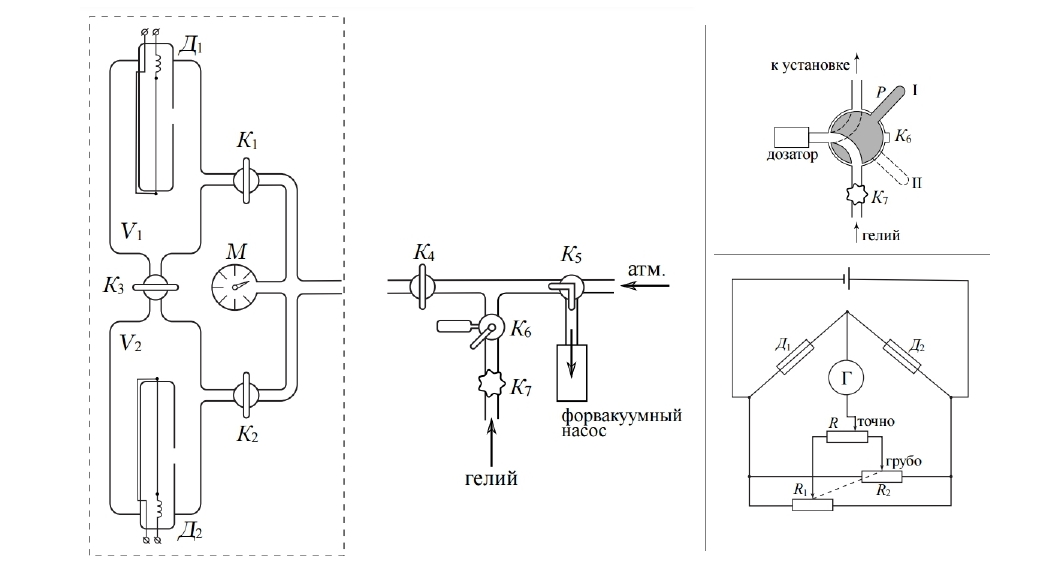
\includegraphics[scale=0.9]{fig1.jpg}}
	\caption{схема установки}
\end{figure}
Установка состоит из двух сосудов $V_1$ и $V_2$ соединенных краном $К_3$, форвакуумного насоса Ф.Н. с выключателем $Т$, манометра $M$ и системы напуска гелия, включающей в себя краны $К_6$ и $К_7$. Кран $К_5$ позволяет соединять форвакуумный насос либо с установкой, либо с атмосферой. Между форвакуумным насосом и краном $К_5$ вставлен предохранительный баллон П.Б., защищающий кран $К_5$ и установку при неправильной эксплуатации ее от попадания форвакуумного масла из насоса Ф.Н. Сосуды $V_1$ и $V_2$ и порознь и вместе можно соединять как с системой напуска гелия, так и с форвакуумным насосом. Для этого служат краны $К_1$, $К_2$, $К_4$ и $К_5$. Манометр  $M$
регистрирует давление газа, до которого заполняют тот или другой
сосуды.

Для сохранения гелия, а также для уменьшения неконтролированного попадания гелия в установку (по протечкам в кране $К_6$) между
трубопроводом подачи гелия и краном $К_6$ поставлен металлический
кран $К_7$. Его открывают только на время непосредственного заполнения установки гелием. Все остальное время он закрыт.

В силу того, что в сосуд требуется подавать малое давление гелия,
между кранами $К_7$ и $К_4$ стоит кран $К_6$, снабженный дозатором. Дозатор - это маленький объем, который заполняют до давления гелия в трубопроводе, а затем уже эту порцию гелия с помощью крана $К_6$ впускают в установку.

Описание схемы электрического соединения. $Д_1$ и $Д_2$ — сопротивления проволок датчиков парциального давления, которые составляют одно плечо моста. Второе плечо моста составляют сопро- тивления $r_1$, $R_1$ и $r_2$, $R_2$. $r_1 \ll R_1$, $r_2 \ll R_2$, $R_1$ и $R_2$ спаренные, их подвижные контакты находятся на общей оси. Оба они исполь- зуются для грубой регулировки моста. Точная балансировка моста выполняется потенциометром R. Последовательно с гальванометром $Г$, стоящим в диагонали моста, поставлен магазин сопротивлений $MR$. Когда мост балансируют, магазин сопротивлений выводят на ноль. В процессе же составления рабочей смеси в сосудах $V_1$ и $V_2$ мост разбалансирован. Чтобы не сжечь при этом гальванометр, магазин $MR$ ставят на максимальное сопротивление.

\section{Ход работы}
Геометрические параметры установки:
\\
\begin{center}
\begin{tabular}{|c|c|c|c|c|}
\hline $V_1, \text{см}^3$, & $V_2, \text{см}^3$ & $L/S, 1/\text{см}$ &
$P_{\text{гел}}$ & $P_{\text{воз}}$ \\
\hline $775 \pm 10$ & $775 \pm 10$ & $5.3 \pm 0.1$ & $0.2 P_{\text{раб}}$ & $1.675 P_{\text{раб}}$ \\ \hline
\end{tabular}
\end{center}
Для каждого из давлений построим графики, откладывая по оси абсцисс время, а по оси ординат --- логарифм от показаний гальванометра и находём угловые коэффициенты каждой прямой:
\begin{figure}[h]
	\center{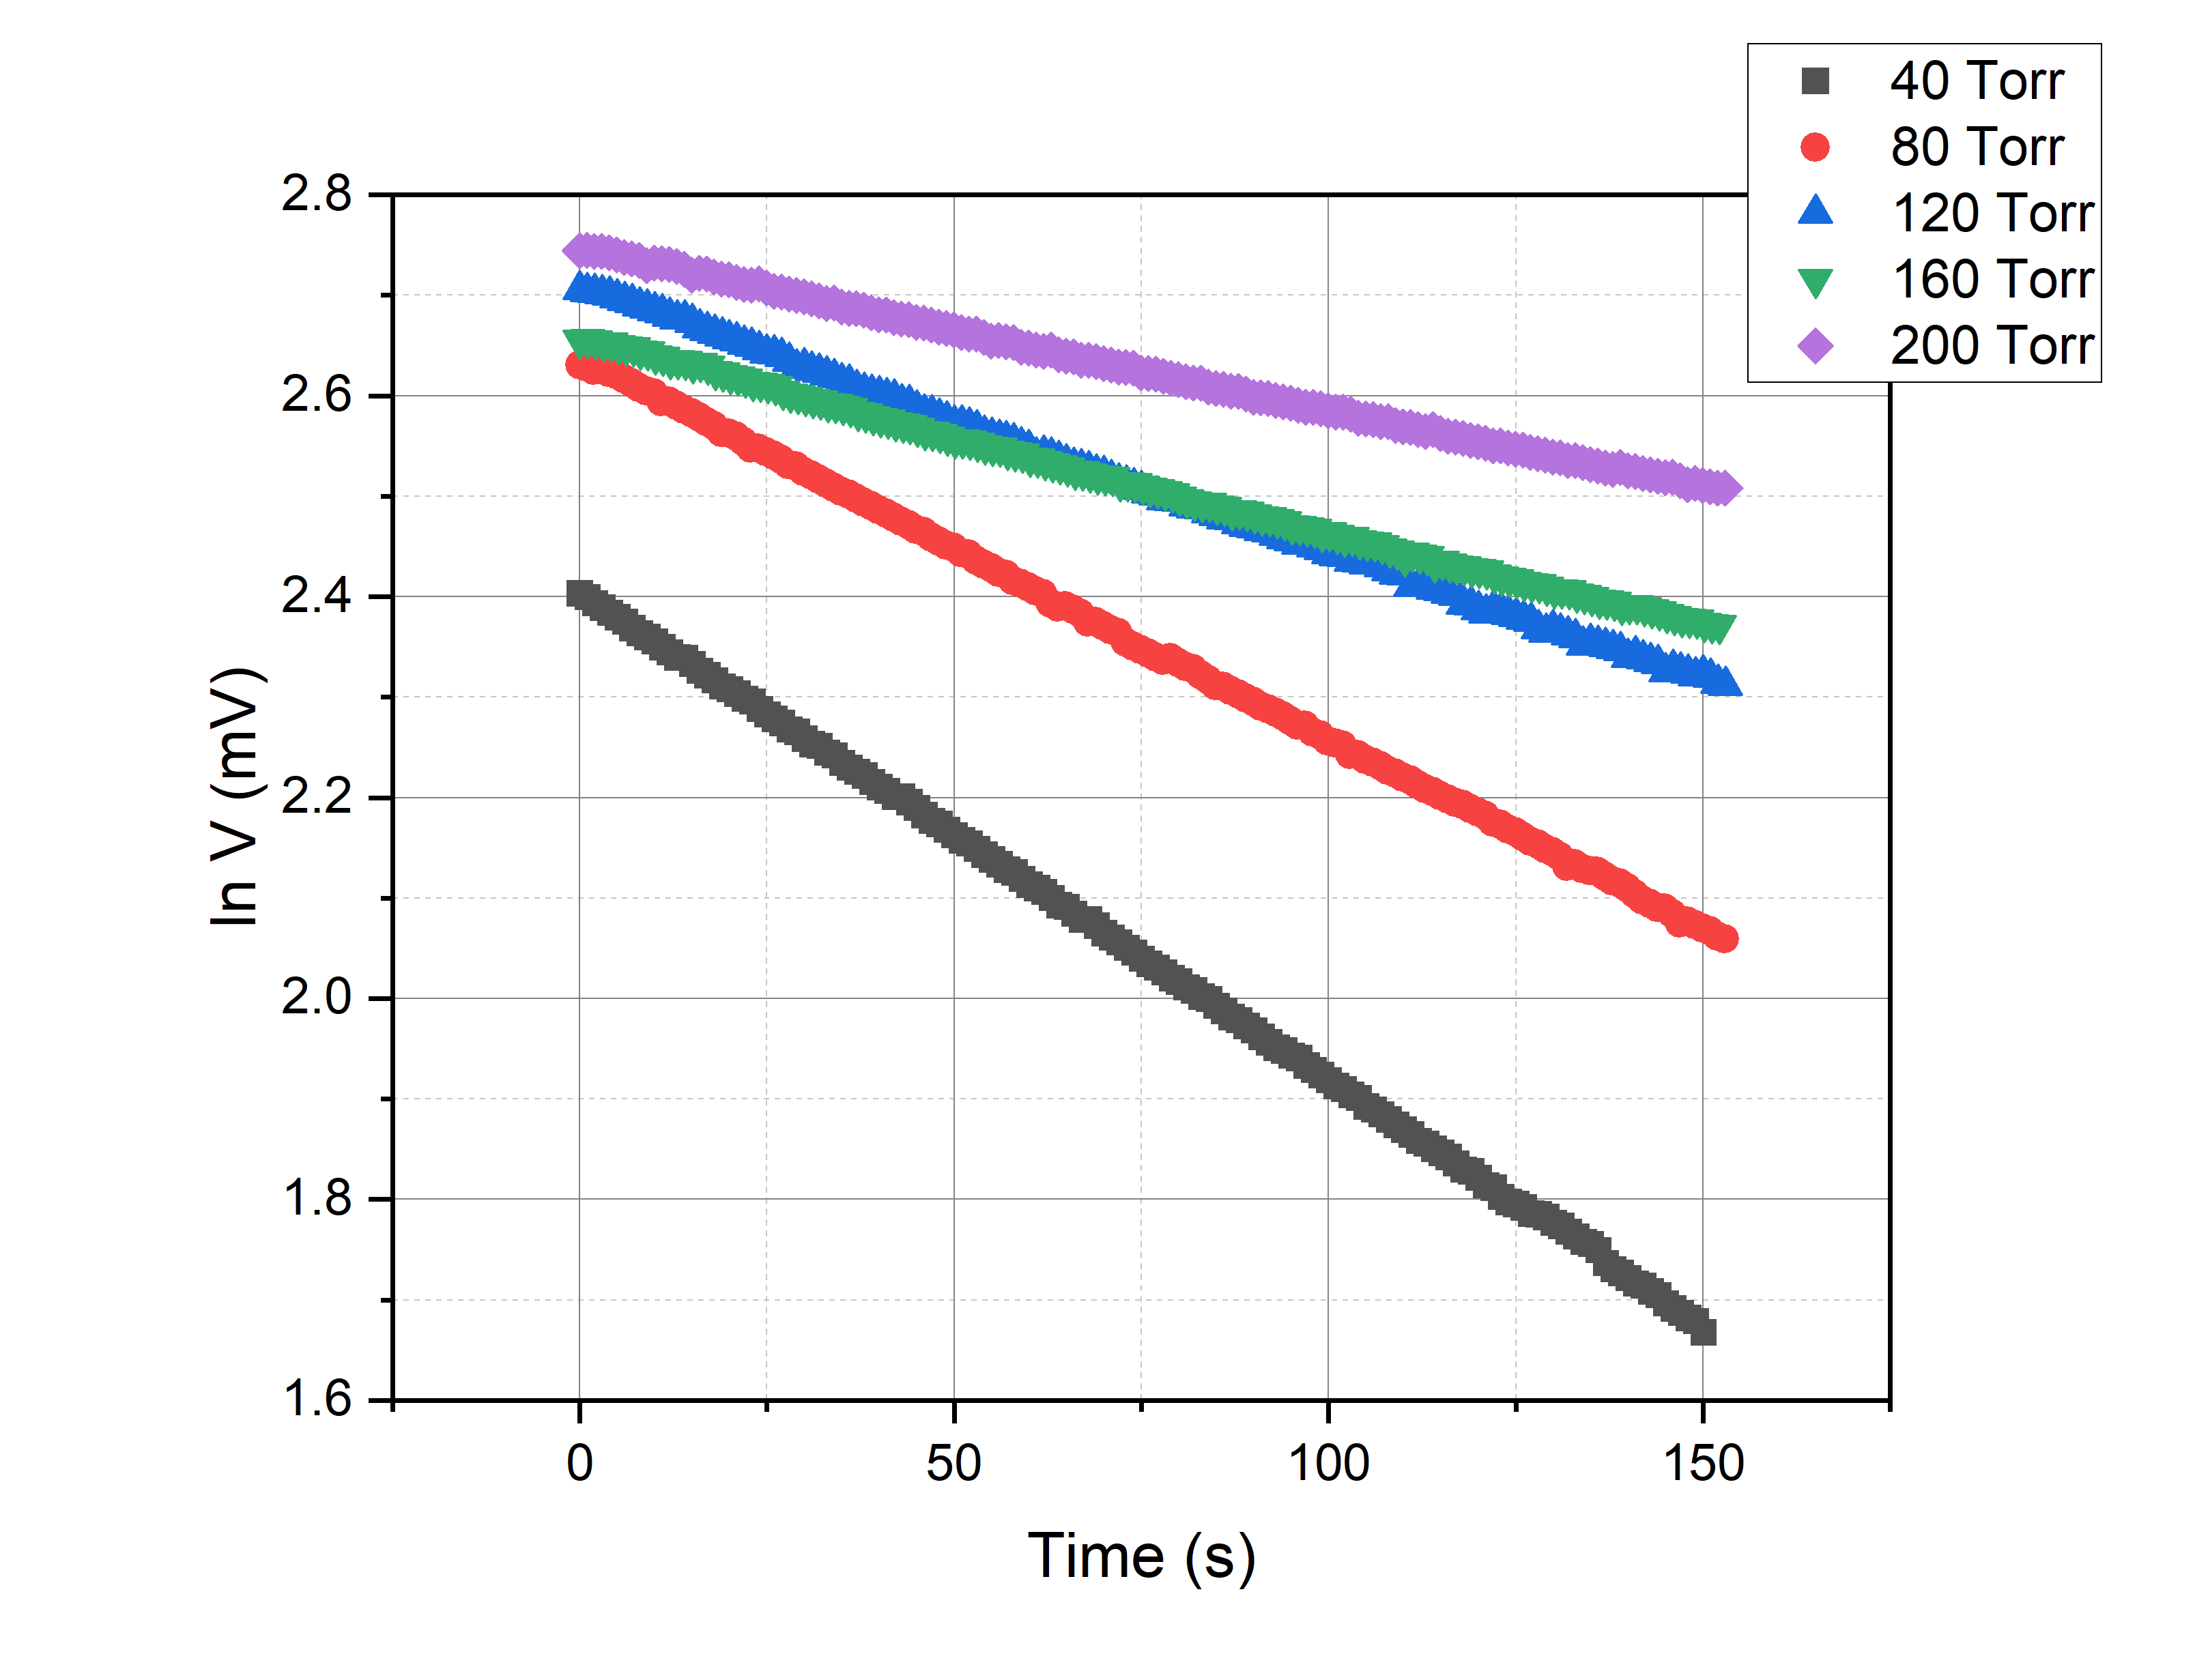
\includegraphics[scale=0.7]{labphoto14}}
	\caption{графики зависимости lnV(t)}
\end{figure}
\linebreak
Угловые коэффициенты графиков:
\begin{center}

\begin{tabular}{|c|c|c|c|c|}
\hline $1/\tau_1,\ 10^{-3} 1/c$ & $1/\tau_2,\ 10^{-3} 1/c$ & $1/\tau_3,\  10^{-3} 1/c$ & $1/\tau_4,\ 10^{-3} 1/c$ & $1/\tau_5,\ 10^{-3} 1/c$ \\
\hline $4.87 \pm 0.05$ & $3.79 \pm 0.03$ & $2.63 \pm 0.03$ &  $1.91 \pm 0.02$ & $1.59 \pm 0.3$ \\\hline
	\end{tabular}
\end{center}

 Найдём коэффициенты взаимной диффузии газов при выбранных давлениях из формулы (2):
 \[
  D=\frac{L}{S} \cdot \frac{V_1V_2}{V_1+V_2} \cdot \frac{1}{\tau}
  \]
\begin{center}
\begin{tabular}{|c|c|c|c|c|}
\hline $D_1,\ \frac{\text{см}^2}{c}$ & $D_2,\ \frac{\text{см}^2}{c}$ & $D_3,\ \frac{\text{см}^2}{c}$ & $D_4,\ \frac{\text{см}^2}{c}$ & $D_5,\ \frac{\text{см}^2}{c}$ \\
\hline $11.13 \pm 0.5$ & $8.66 \pm 0.5$ & $5.99 \pm 0.5$ &  $4.51 \pm 0.5$ & $3.64 \pm 0.5$ \\\hline
	\end{tabular}
\end{center}
Построим график зависимости $D(\frac{1}{P})$ и по его коэффициенту наклона рассчитаем величину коэффициента диффузии при атмосферном давлении:
\begin{figure}[h]
	\center{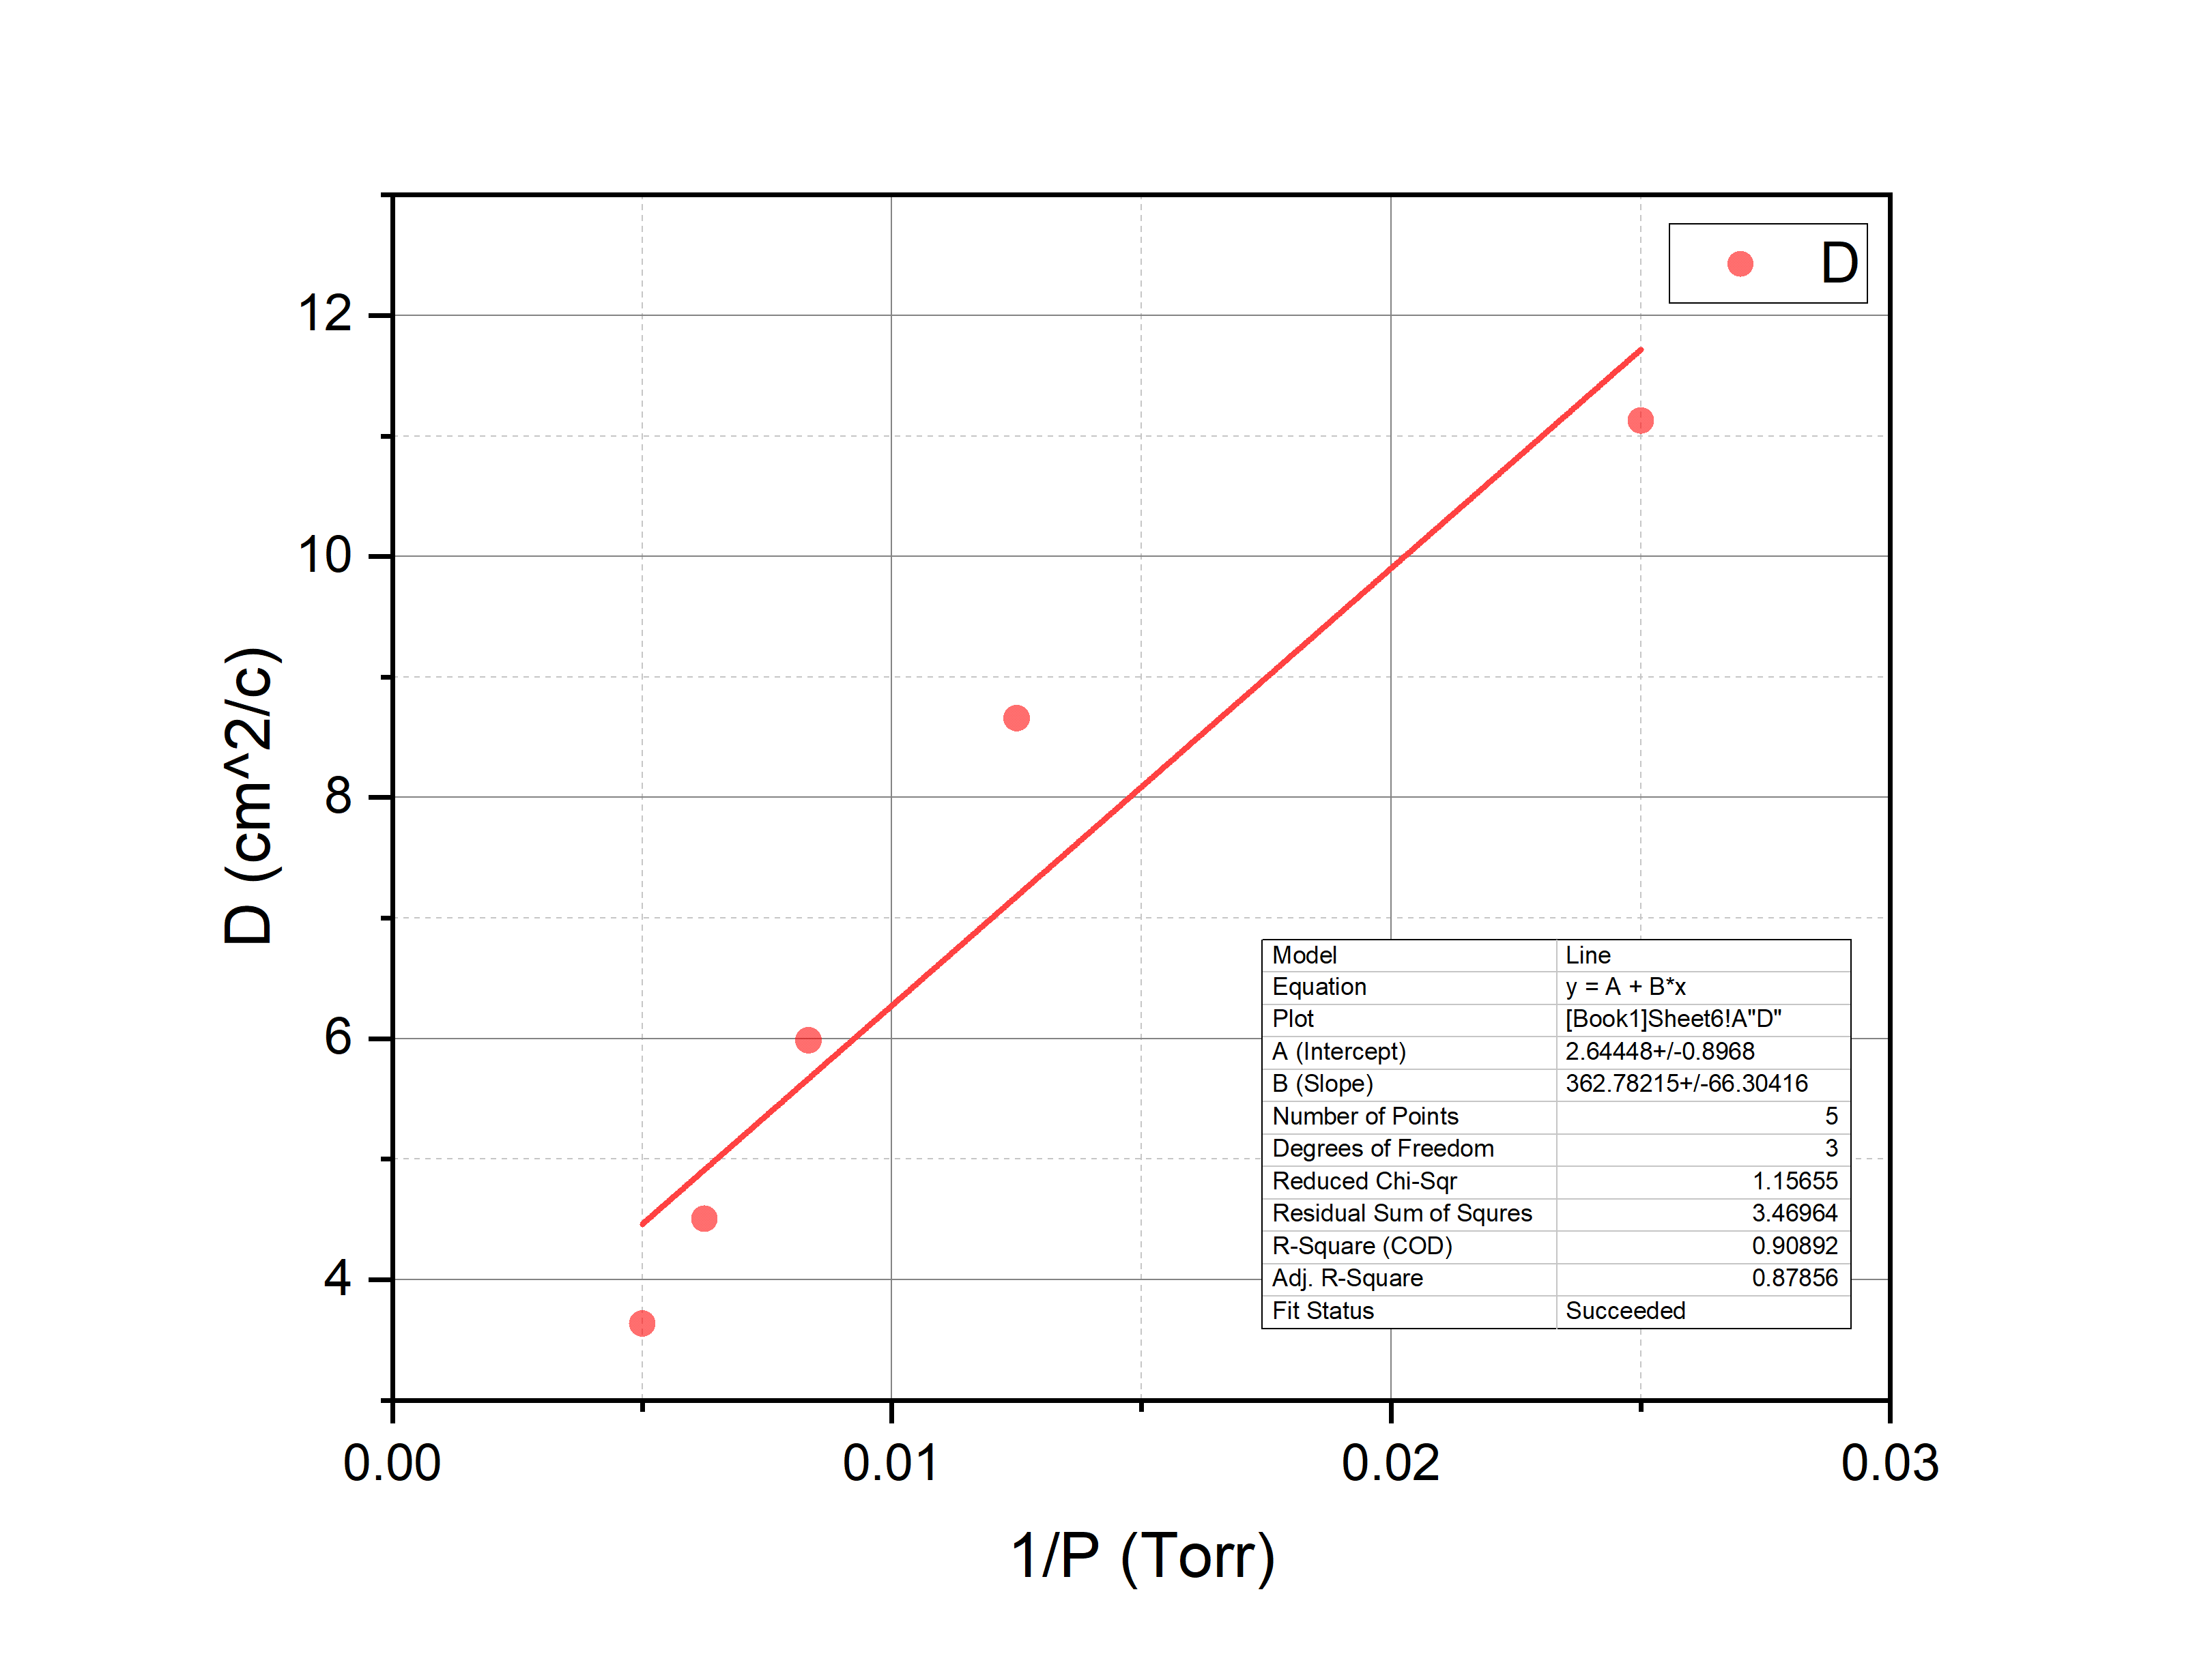
\includegraphics[scale=0.7]{labphoto16}}
	\caption{График зависимости $D(\frac{1}{P})$}
\end{figure}

Проведём аппроксимацию полученной зависимости прямыми $ y =kx + b $ методом Йорка, который учитывает погрешность $ \sigma_{1/P}, $ при помощи программы OriginPro 2022. В итоге получаем \[ k = (362,78 \pm 25,8) \text{ } \frac{\text{см}^2}{\text{с}\cdot\text{торр}}. \]

Таким образом, для атмосферного давления в экспериментальной дате ($ P=752 $ торр) получаем \[ \boxed{D_\text{атм} = (0,48\pm0,05) \text{ } \frac{\text{см}^2}{\text{с}}}, \quad \]


\section{Вывод}

В итоге, для коэффициента взаимной диффузии смеси гелий-воздух мы получили:

\[ \boxed{D_\text{атм} = (0,48\pm0,03) \text{ } \frac{\text{см}^2}{\text{с}}}, \quad (\varepsilon = 8.3\%). \]

Сравним полученные данные с табличными. Из таблицы в <<Лабораторном практикуме>> имеем:

\[ D_\text{табл} = 0,58 \text{ } \frac{\text{см}^2}{\text{с}}. \]

Таким образом, полученные экспериментально данные отличаются от табличных и не совпадают в пределах погрешности. Однако, полученные результаты совпадают с табличным значением по порядку величины, что может говорить об их качественной достоверности. Полученное экспериментально значение позволяет качественно описать процесс взаимной диффузии смеси воздух-гелий, а отклонение от табличного значения могло возникнуть из-за неидеальных условий проведения эксперимента. Так, не удавалось точно добиться необходимого начального давления, тем самым нарушалась балансировка моста и измерения могли исказиться.

Также были оценены длина свободного пробега гелия в воздухе и сечение столкновения его атомов с молекулами воздуха. Мы получили:

\[ \boxed{\lambda = (107,3 \pm 7,5) \text{ нм}}, \quad (\varepsilon = 7\%),\]

\[ \boxed{\sigma \approx (3,51 \pm 0,24) \cdot 10^{-19} \text{ м}^2}, \quad (\varepsilon = 7\%).\]

Сравним полученные данные с табличными. Из справочников имеем:

\[ \lambda_\text{табл} = 175 \text{ нм}, \]

\[ \sigma_\text{табл} = 5,89  \cdot 10^{-19} \text{ м}^2.\]

Таким образом, наша оценка по порядку величины совпадает с табличными данными.




\end{document}